
\section{Synthetic Single-Task Benchmark with Model Mismatch}
\label{section:exp_model_mismatch}

\begin{figure*}
\centering
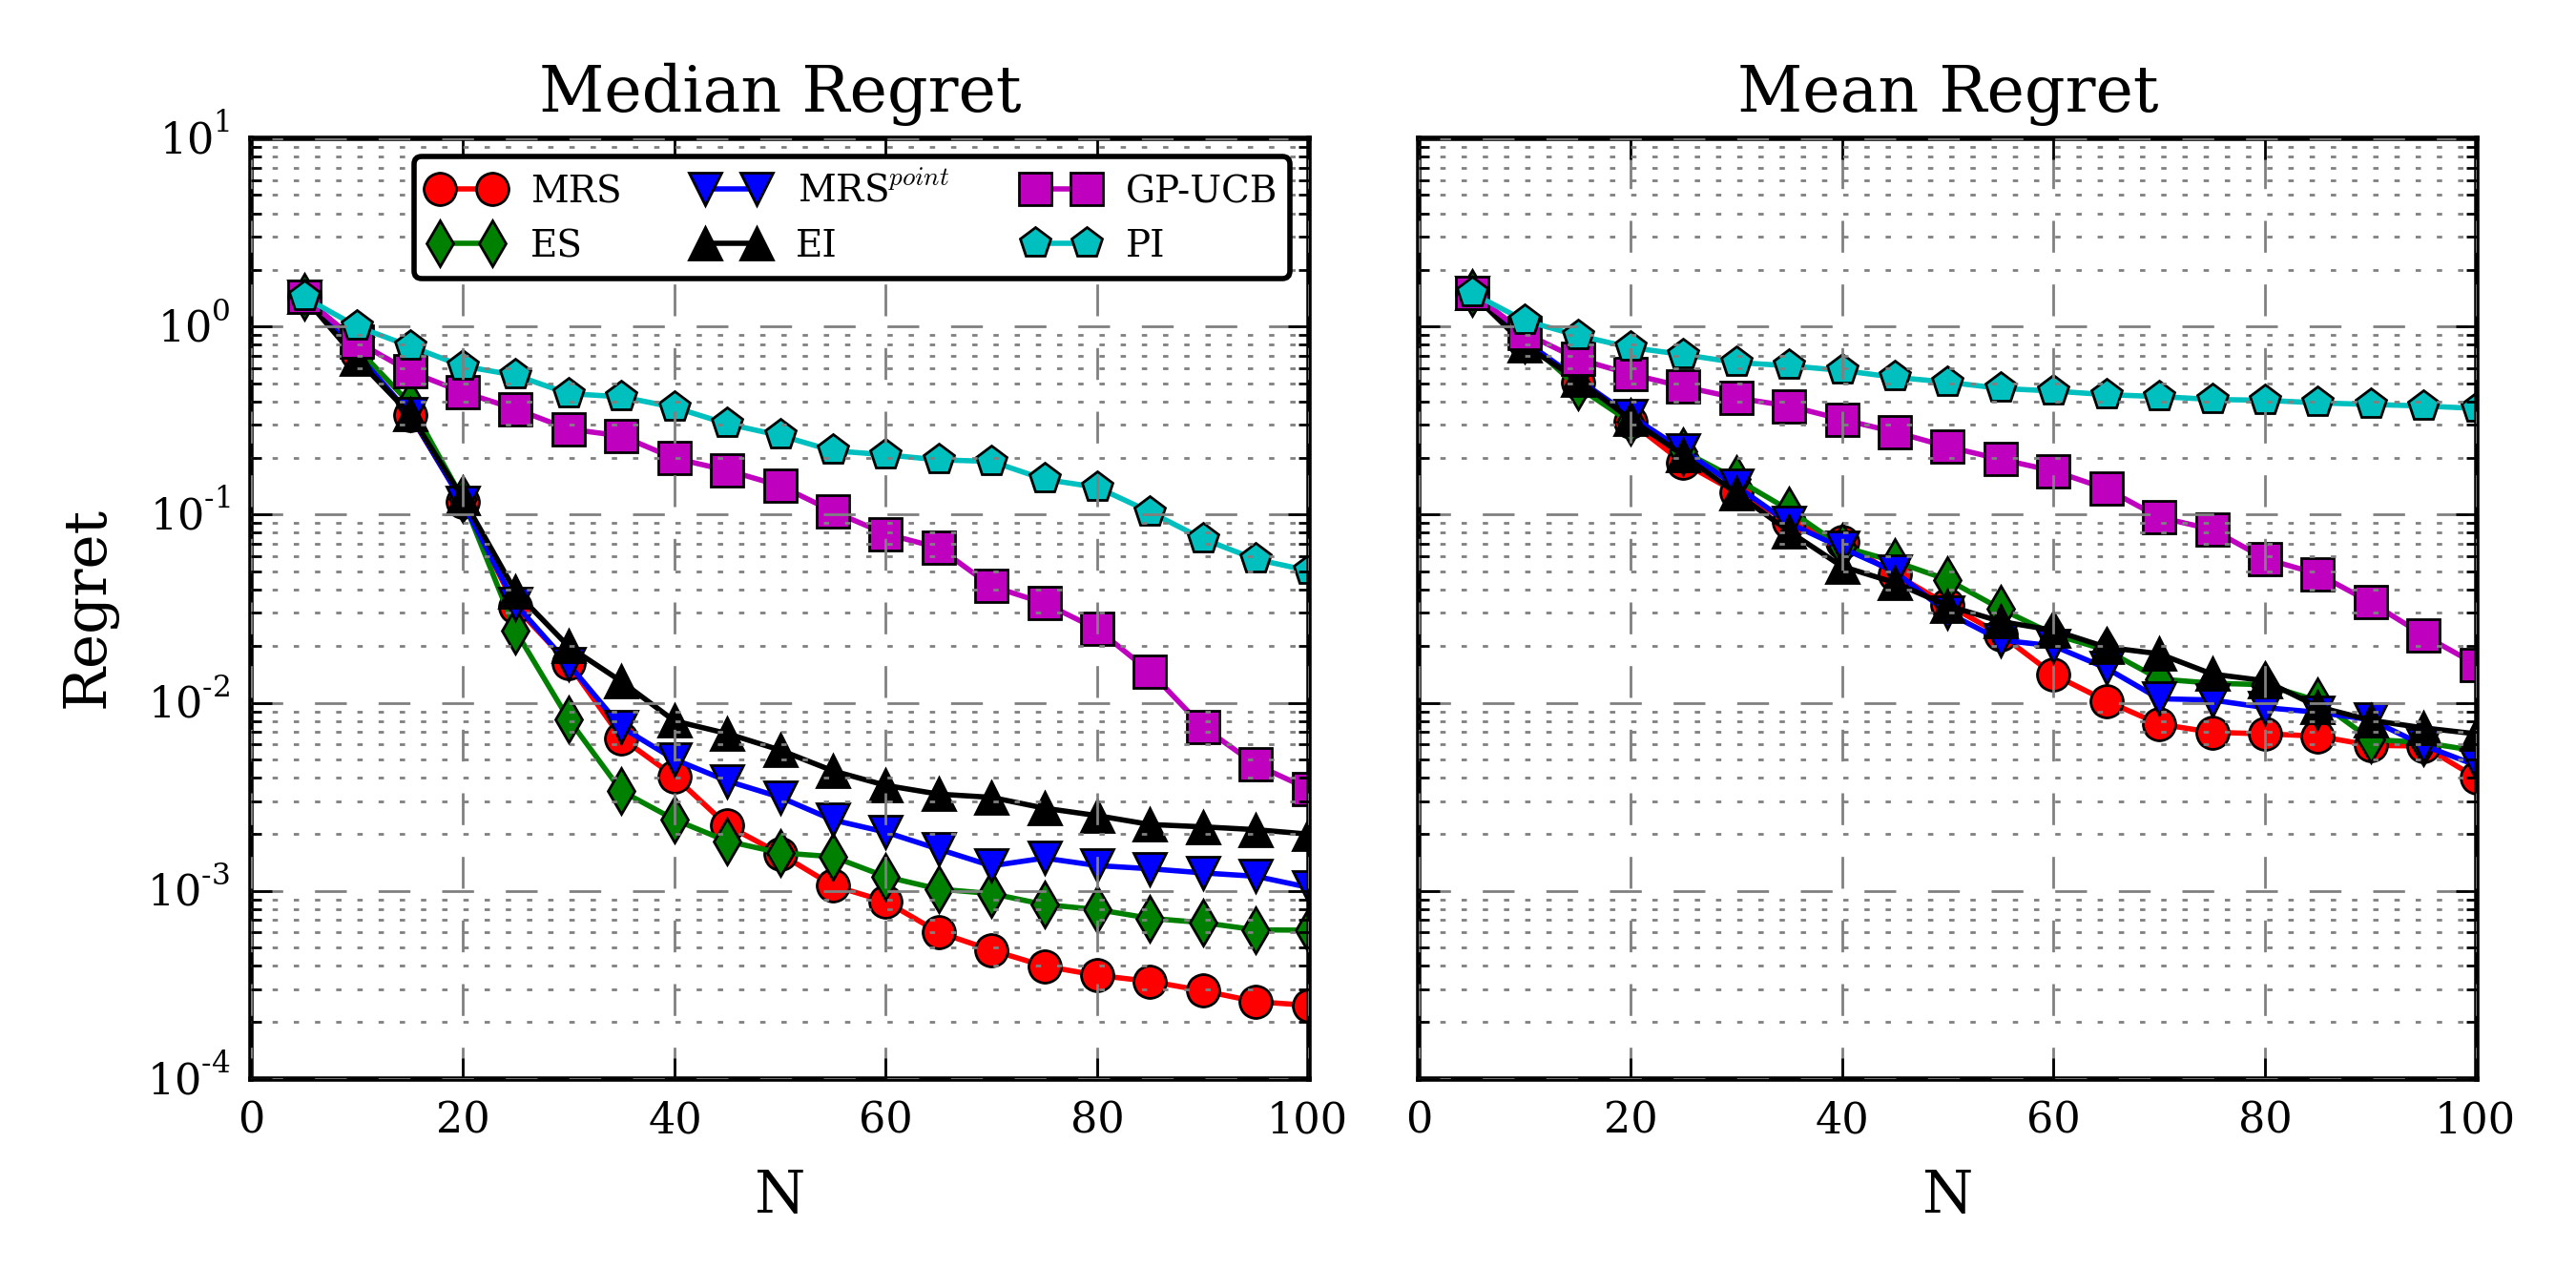
\includegraphics[width=.9\textwidth]{empirical_comparison_mm}
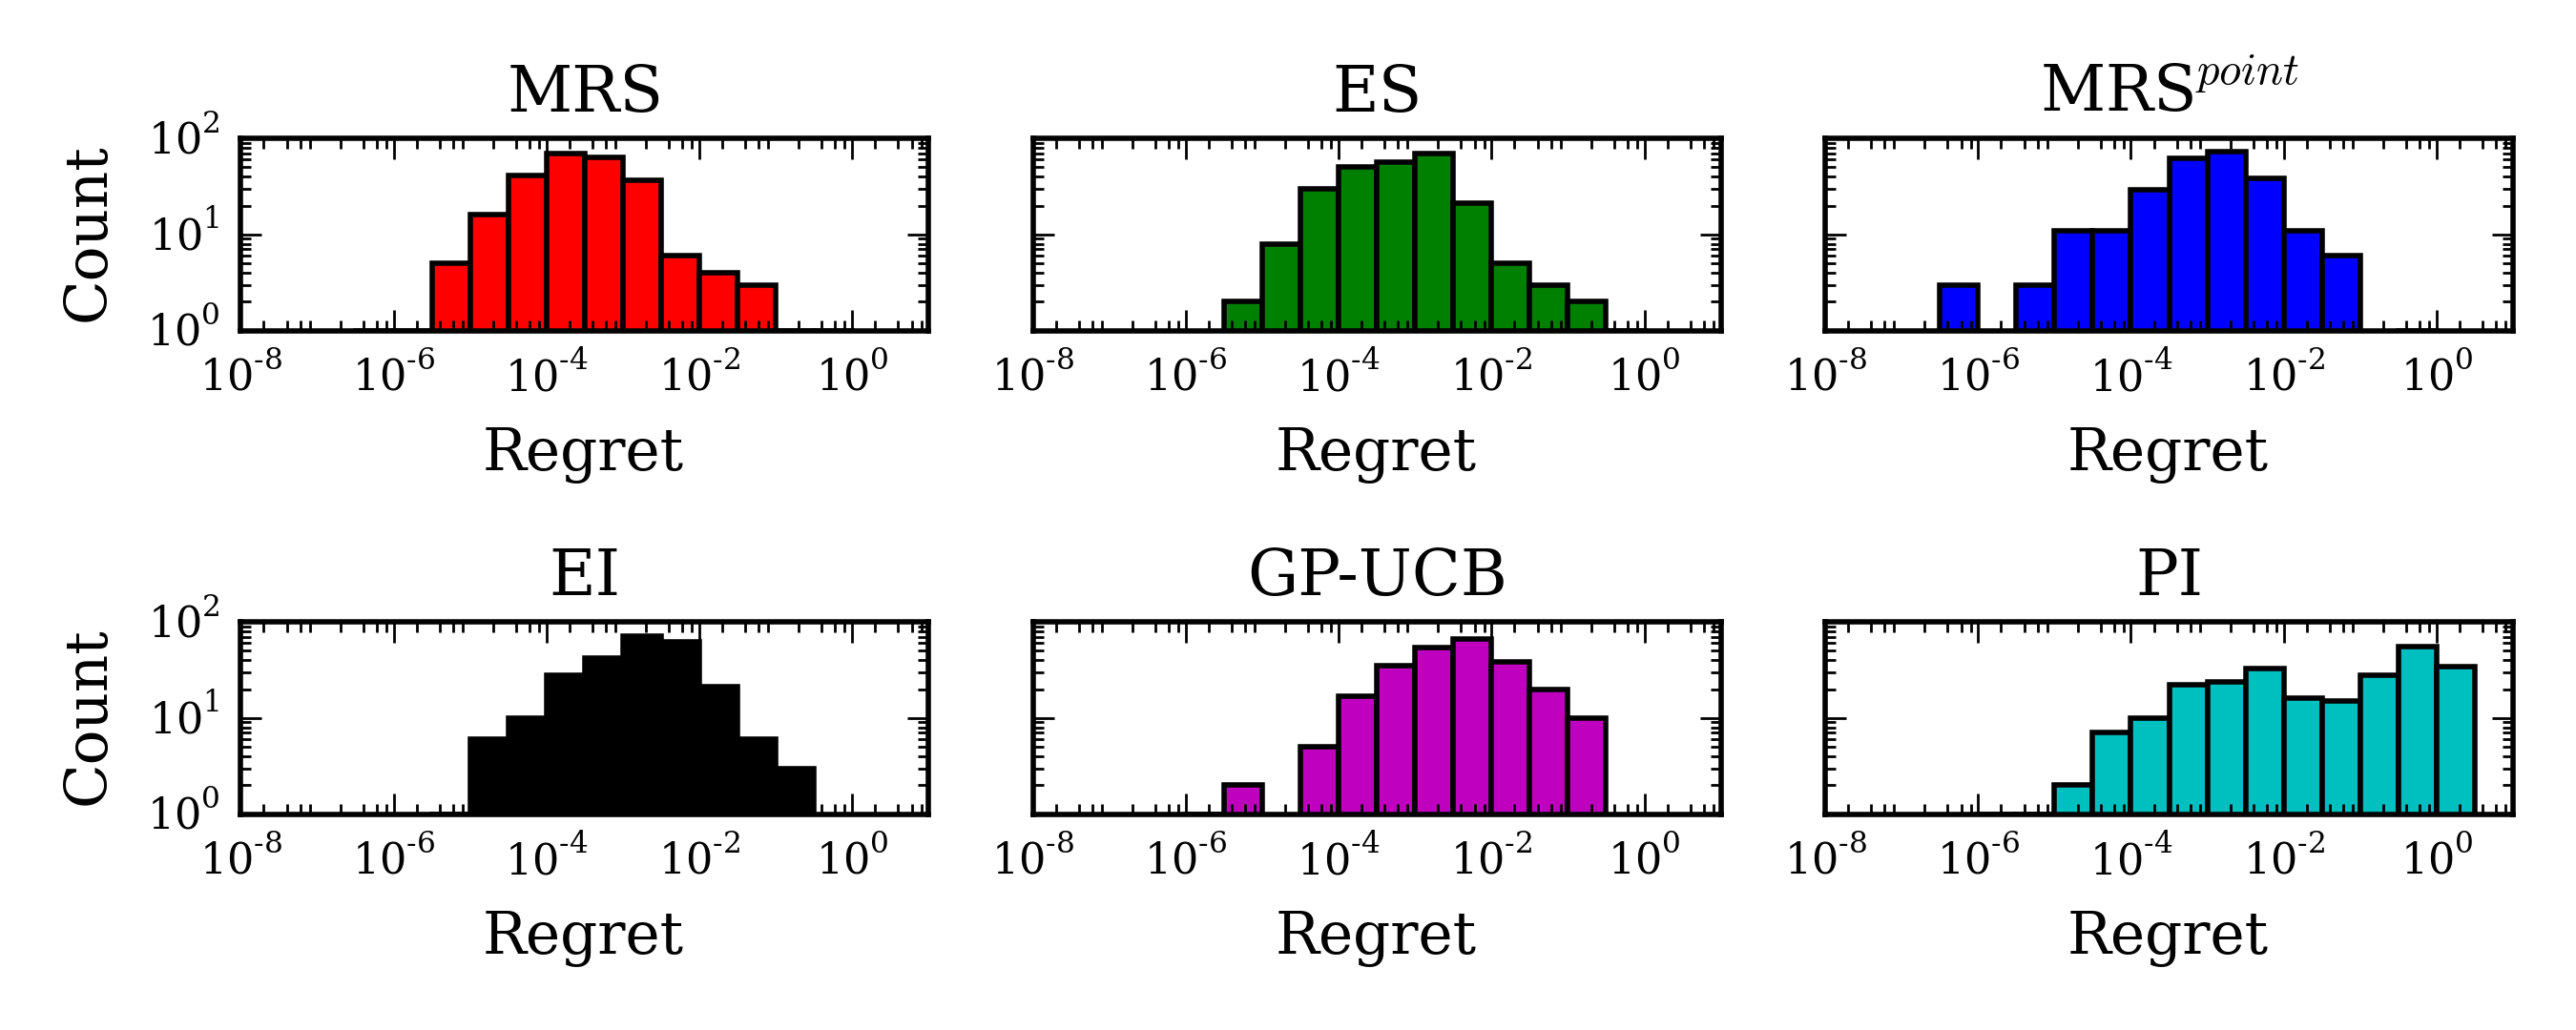
\includegraphics[width=.9\textwidth]{hist_mm}
\caption{(Top) Median and mean simple regret over $250$ repetitions for different acquisition functions. Shown is the simple regret of the recommendation $\mathbf{\tilde x}_N$ after $N$ trials, i.e., the point which maximizes the GP posterior
mean. (Bottom) Histogram of the simple regret after performing $N=100$ trials for different acquisition functions (note the log-scales).}
\label{fig:empirical_comparison_mm}
\end{figure*}

We present results for an identical setup as reported in Section \ref{Section:ResultsSingleTask},
with the
only difference being that the test functions have been sampled from a GP with
rational quadratic kernel with length scale $l=0.1$ and scale mixture
$\alpha=1.0$. The kernel used in the GP surrogate model is not modified, i.e.,
an RBF kernel with length scale $l=0.1$ is used. Thus, since different kind of
kernel govern test functions and surrogate model, we have model mismatch as
would be the common case on real-world problems. Figure
\ref{fig:empirical_comparison_mm} summarizes the results of the experiment.
Interestingly, in contrast to the experiment without model mismatch, for this setup
there are also considerable differences in the mean simple regret between MRS
and ES: while ES performs slightly better initially, it is outperformed by MRS
for $N > 60$. We suspect that this is because ES tends to explore more locally
than MRS once $p^\star$ has mostly settled onto one region of the search
space. More local exploration, however, can be detrimental in the case of
model-mismatch since the surrogate model is more likely to underestimate the
function value in regions which have not been sampled. Thus a more homogeneous
sampling of the search space as done by the more global exploration of MRS is
beneficial. As a second observation, in contrast to a no-model-mismatch
scenario, MRS$^\text{point}$ performs considerably worse than MRS when there
is model-mismatch. This emphasizes the importance of accounting for
uncertainty, particularly when there is model mis-specification.

According to the median simple regret, the difference between MRS,
MRS$^\text{point}$, ES, and EI is less pronounced in Figure
\ref{fig:empirical_comparison_mm}. Moreover, the histograms of the regret
distribution exhibit less outliers (regardless of the method). We suspect that
this stems from properties of the test functions that are sampled from a GP
with rational quadratic rather than from the model-mismatch. However,
a conclusive answer on this would require further experiments.

